\newpage
\subsection{Stereo reconstruction from VHR optical image pair}\label{sec:stereoreconstruction}

This section describes how to convert pair of images into elevation information.

The standard problem of terrain reconstruction with \app presented here contains
the following steps:

\begin{itemize}
\item Estimation of displacements grids for epipolar geometry transformation
\item Epipolar resampling of the image pair using those grids
\item Dense disparity map estimation
\item Projection of the disparities on a Digital Elevation Map (DEM)
\end{itemize}

%tenez vous pret?
Let's go now to the third dimensions!

\subsubsection{First step: Estimate epipolar geometry transformation}\label{ssec:epipolar}
The aim of this application is to generate resampling grids to transform images
in epipolar geometry.  Epipolar geometry is the geometry of stereo vision (see
\href{http://en.wikipedia.org/wiki/Epipolar_geometry}{here}). The operation of stereo
rectification determines a transformation of each image such that pairs of
conjugate epipolar lines become collinear and parallel to one of the image axes.

After applying this transformation, it reduces the problem of elevation (or
stereo correspondences determination) to a 1-D problem.  We've got two images
image1 and image2 over the same area (the stereo pair) and we assume that we
know the localization functions (forward and inverse) associated for each of
these images.

The forward function allows to go from the image referential to the geographic
referential:
\begin{equation}
  (long,lat) = f^{forward}_{image1}(i,j,h)
\end{equation}

where h is the elevation hypothesis, $(i,j)$ are the pixel coordinates in image1
and (long,lat) are geographic coordinates. As you can imagine, the inverse
function allows to go from geographic coordinates to the image geometry.

For the second image:

\begin{equation}
   (long,lat,h) = f^{inverse}_{image2}(i,j)
\end{equation}

Using jointly the forward and inverse functions from the image pair, we can
construct a co-localization function $f_{image1 \rightarrow image2}$ between
the position of a pixel in the first and its position in the second one:

\begin{equation}
(i_{image2},j_{image2}) = f_{image1 \rightarrow image2} (i_{image1} , j_{image1} , h)
\end{equation}

The expression of this function is:

\begin{equation}
f_{image1 \rightarrow image2} (i_{image1} , j_{image1} , h) =  f^{inverse}_{image2} f^{forward}_{image1}((i_{image1} , j_{image1}), h)
\end{equation}

The expression is not really important, what we need to understand is that if we
are now able to determine for a given pixel in image1 the corresponding pixel in
image2.As we know the expression of co-localization function between images,as a
result we've got the information about the elevation (variable h in the
equation)!

We've got now the mathematical basis to understand how 3-D information can be
extracted by examination of the relative positions of objects in the two 2-D
epipolar images.

The construction of the two epipolar grids is a little bit more complicated in
case of VHR optical images.That's because most of passive remote sensing from
space use a push-broom sensor, which corresponds to a line of sensors arranged
perpendicular to the flight direction of the spacecraft.  This acquisition
configuration implies a slightly different strategy for stereo-rectification
(see
\href{http://en.wikipedia.org/wiki/Epipolar_geometry#Epipolar_geometry_of_pushbroom_sensor}{here}).

Let's examine now how to use the \application{StereoRectificationGridGenerator}
application to produce two images which are \textbf{deformation grids} for
the two images.

\begin{verbatim}
otbcli_StereoRectificationGridGenerator -io.inleft image1.tif
                                        -io.inright image1.tif
                                        -epi.elevation.avg.value 50
                                        -epi.step 5
                                        -io.outimage1 outimage1_grid.tif
                                        -io.outright outimage1_grid.tif
\end{verbatim}

The application estimates the displacement to apply for each pixel in the two
input images to obtain epipolar geometry.You can see that the application can
accept a `step' parameter to estimate displacements on a coarser grid. Here we
estimate the displacements every 10 pixels. That's because in most cases with a
pair of VHR and a small angle between the two images, this grid is almost
regular.Moreover, the implementation is not \textit{streamable} and use potentially a
lot of memory. So that, it is generally a good idea to estimate the displacement
grid at a coarser resolution.

The application outputs the size of the output image in epipolar
geometry. \textbf{Note these values}, we will use it at the next step to
resample the two images in epipolar geometry.

In my case, I've got:

\begin{verbatim}
Output parameters value:
epi.rectsizex: 4462
epi.rectsizey: 2951
epi.baseline: 4.7746
\end{verbatim}

The epi.baseline parameter provides the mean value(in meters) of the
baseline to sensor altitude ratio. It can be used to convert disparities to
physical elevation, since a disparity of one pixel will correspond to an
elevation offset of this value with respect to the mean elevation.

Let's move forward to the resampling in epipolar geometry.

\subsubsection{Resample images in epipolar geometry}

The prior application generates two grids of displacements. The
\application{GridBasedImageResampling} allows to resample the two input images
in the epipolar geometry using these grids.  These grids are intermediary result
not really useful as it in most cases. This second step \textit{only} consists in
applying the transformation and resample both images but this application can be
useful in a lot of other cases.

The two commands to generate epipolar images are:
\begin{verbatim}
otbcli_GridBasedImageResampling -io.in image1.tif
                                -io.out image1_epipolar.tif
                                -grid.in outimage1_grid.tif
                                -out.sizex 4462
                                -out.sizey 2951
\end{verbatim}

\begin{verbatim}
otbcli_GridBasedImageResampling -io.in image2.tif
                                -io.out image2_epipolar.tif
                                -grid.in outimage2_grid.tif
                                -out.sizex 4462
                                -out.sizey 2951
\end{verbatim}

As you can see, we set \textit{sizex} and \textit{sizey} parameters using output values given by
the \application{StereoRectificationGridGenerator} application to set the size
of the output epipolar images.

\begin{figure}[!h]
  \center
  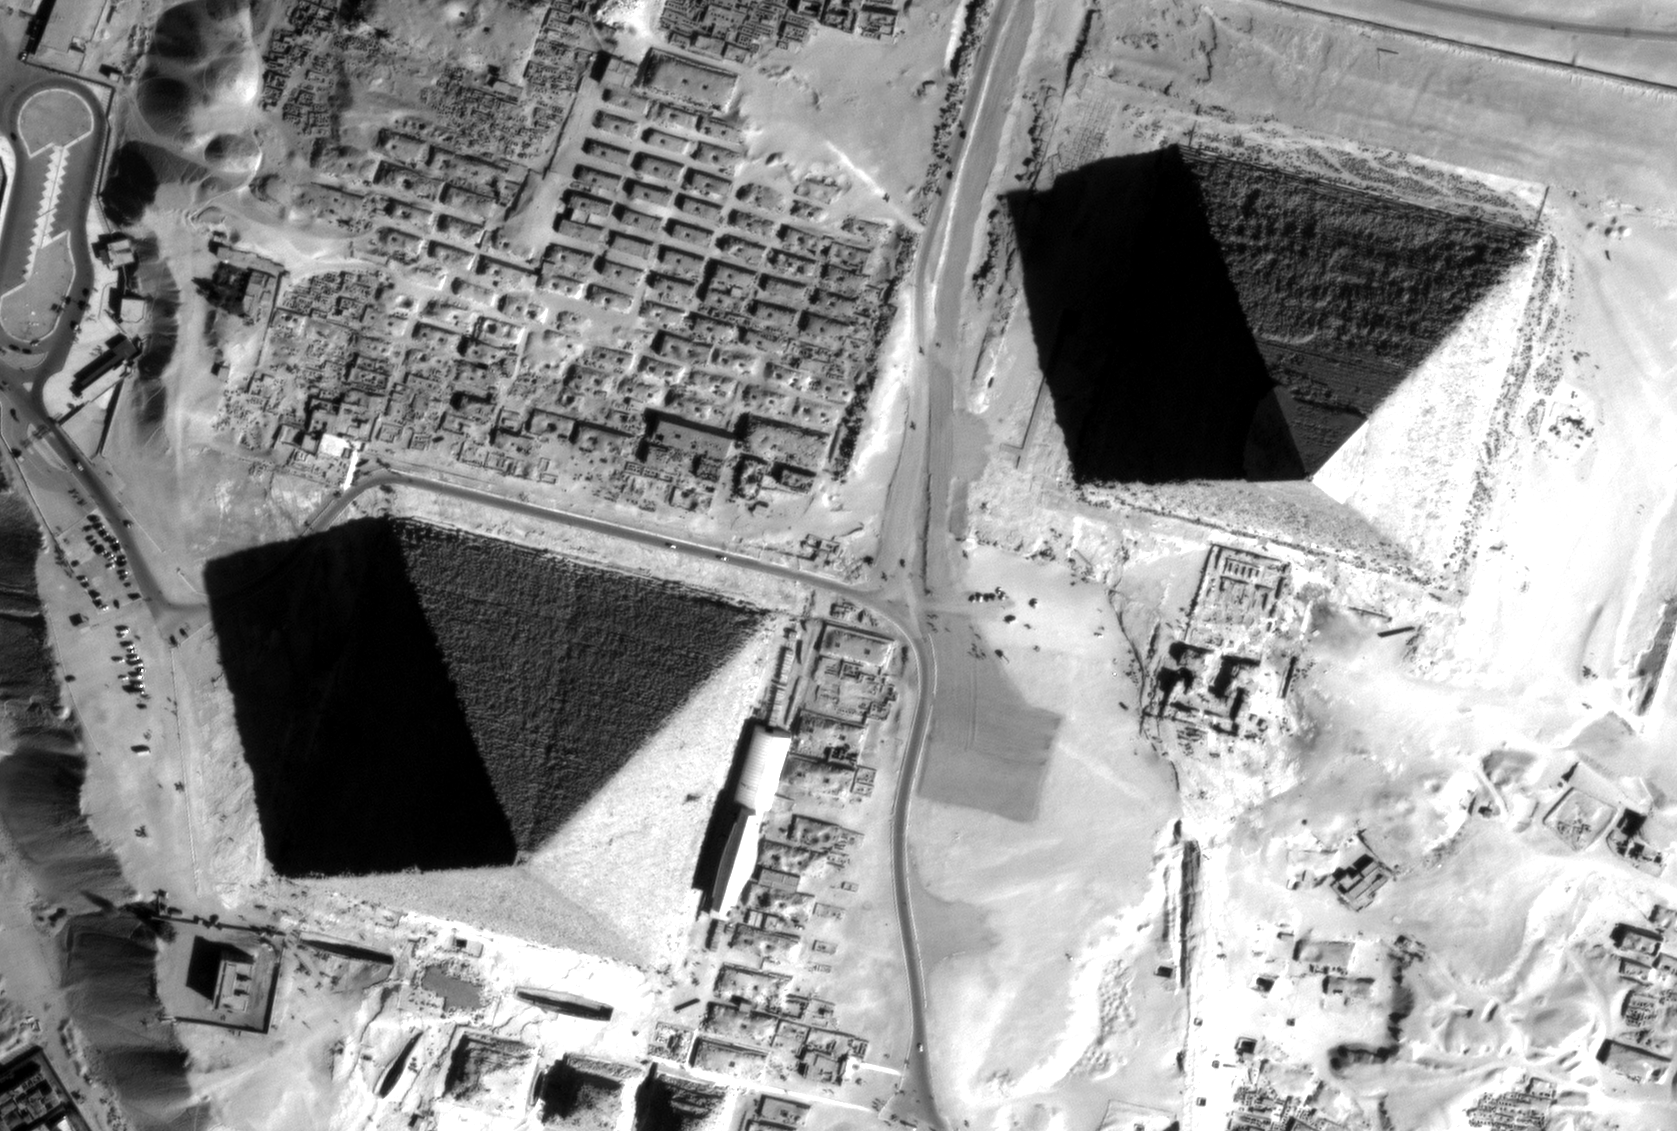
\includegraphics[width=0.45\textwidth]{../Art/MonteverdiImages/stereo_image1_epipolar.png}
  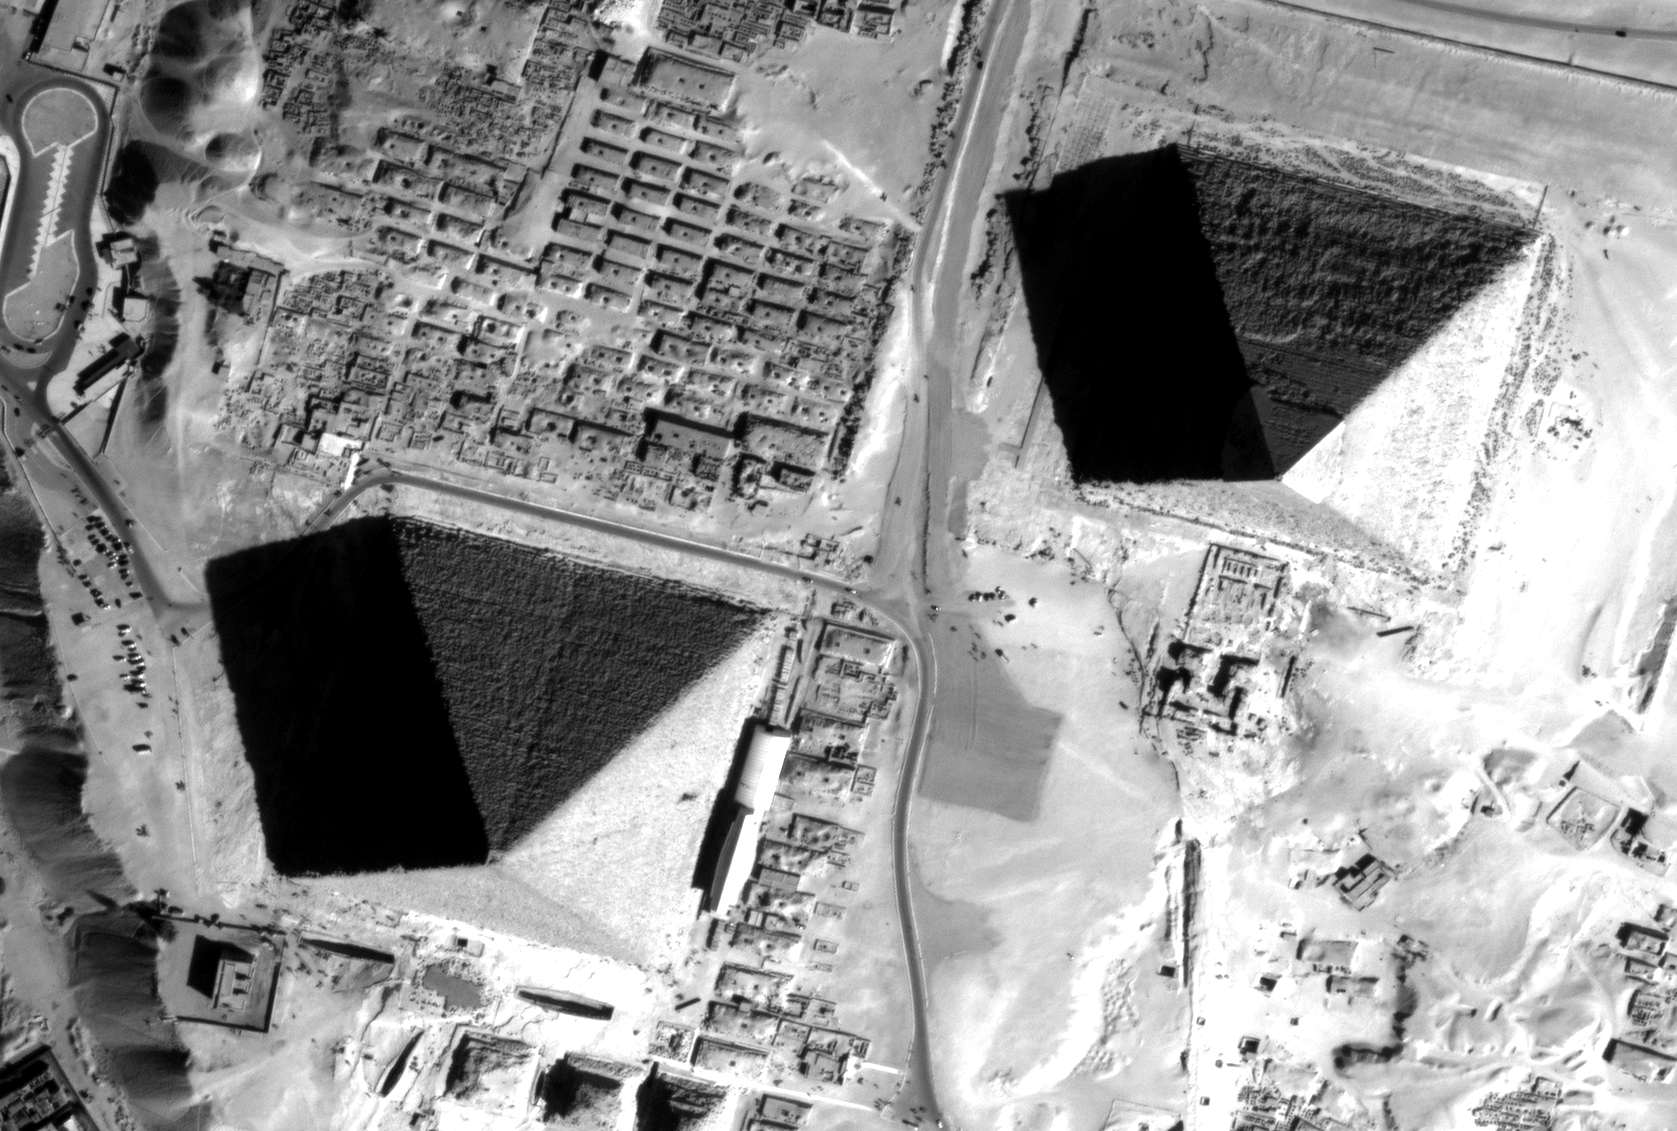
\includegraphics[width=0.45\textwidth]{../Art/MonteverdiImages/stereo_image2_epipolar.png}
  \itkcaption[ExampleEpipolar]{Extract of resample image1 and image2 in epipolar
    geometry over Pyramids of Cheops.}
  \label{fig:MeanShiftVectorImageFilter}
\end{figure}

\subsubsection{Disparity estimation: Block matching on epipolar lines}

Finally, we can begin the stereo correspondences!

Things become a little bit more complicated but don't worry and lets describe
now the powerfulness of the \application{BlockMatching} application.

To correlate block from the first image with a block in the second image, we've
got two epipolar data where the use of epipolar lines allows us to constrain the
search along a 1-dimensional line as opposed to the entire 2-dimensional
image. Moreover, block matching is used, as opposed to single point matching,
because of the obvious advantage that correlating blocks is much more likely to
reflect a true match.

For each point in the first image (the \textit{baseline}), we can search for the
corresponding pixel in the second image and use the co-localization function
describes in \ref{ssec:epipolar}.

An almost complete spectrum of stereo correspondence algorithms has been
published and it is still augmented at a significant rate!See for example
\href{http://en.wikipedia.org/wiki/Block-matching_algorithm} for example. The
\otb implements different strategies for block matching:

\begin{itemize}
\item Sum of Square Distances block-matching (SSD)
\item Normalized Cross-Correlation (NCC)
\item Lp pseudo-norm (LP)
\end{itemize}

An other important parameter (mandatory in the application) is the range of
disparities. In theory, the block matching can perform a blind exploration and
search for a infinite range of disparities between the stereo pair. We need now
to evaluate the range of disparities where the block (from the deepest point on
Earth, \url{http://en.wikipedia.org/wiki/Challenger_Deep}{the Challenger Deep}.
to the Everest summit!

I deliberately exaggerated but you can imagine that with a smaller range you can
imagine that the block matching algorithm can take a lot of time.  That's why
these parameters are mandatory for the application and as consequence we need to
estimate them manually. That's pretty simple using the two epipolar images.

In my case, I take one point on a flat area. The image coordinate in $image_{1}$
is $[1970,1525]$ and in $image_{2}$ is $[1970,1526]$. I take after that a second
point on a higher region (in my case a point near the top of the Pyramid of
Cheops!). The image coordinate of this pixel in $image_{1}$ is $[1661,1299]$ and
in $image_{2}$ is $[1633,1300]$.  So you see for the vertical exploration, I
must set the minimum value to a minimum $-30$ (the convention for the sign of the
disparity range is from image1 to image2).

Note that, this estimation can be facilitate using an external DEM in the
\application{StereoRectificationGridGenerator} application.Concerning the
vertical disparity, in the first step we said that we reduce the problem of 3D
extraction to a 1D problem, that's not completely true in general cases. In our
case, there are small disparities in the vertical direction which are due to
parallax errors (i.e. epipolar lines exhibit a small shift in the vertical
direction, around 1 pixel). So that, exploration in the vertical direction of
disparities are so typically smaller than horizontal one. You can also estimate
them on the epipolar couple (in my case I use a range of $-1$ to $1$).

One more time take care of the sign of this minimum and this maximum for
disparities (always from image1 to image2).

The command line for the \application{BlockMatching} application is :
\begin{verbatim}
otbcli_BlockMatching -io.inleft image1_epipolar.tif
                     -io.inright image2_epipolar.tif
                     -io.out disparity_map_ncc.tif
                     -bm.minhd -45
                     -bm.maxhd 5
                     -bm.minvd 1
                     -bm.maxvd 1
                     -mask.nodata 0
                     -mask.variancet 10
                     -io.outmetric 1
                     -bm.metric ncc
                     -bm.subpixel dichotomy
                     -bm.medianfilter.radius 5
                     -bm.medianfilter.incoherence 2.0
\end{verbatim}

The application creates by default a two bands image : the horizontal and
vertival disparity.

The \application{BlockMatching} application gives access to a lot of other
powerful functionalities to improve the quality of the disparity.

Let's describe now these functionalities:

\begin{itemize}
\item -io.outmetric : Output the metric:if the optimal metric values image is
  activated, it will be concatenated to the output image (which will then
  have three bands : horizontal disparity, vertical disparity and metric value)
\item -bm.subpixel : Perform sub-pixel estimation of disparities
\item -mask.nodata 0 : as a consequence, you can specify a no-data value which
  will discard pixels with this value (for example the epipolar geometry can
  generate large part of images with black pixels)
\item -mask.variancet : The block matching algorithm have difficulties to find
  matches on uniform zone. We can use the variance threshold to discard those
  regions and speed-up again computation time.
\item -bm.medianfilter.radius 5 and -bm.medianfilter.incoherence 2.0 : Applies a
  median filter to the disparity map. A median filter is one of the family of
  nonlinear filters.It is used to smooth an image without being biased by
  outliers or shot noise. The radius corresponds to the neighborhood where the
  median value is computed.A detection of incoherences between the input
  disparity map and the median is performed (a pixel corresponds to an
  incoherence if the absolute value of the difference between the pixel value in
  the disparity map and in the median image is higher than the incoherence
  threshold (whose default value is 1).Both parameters must be defined in the
  application to activated the filter.
\end{itemize}

Of course all these parameters can be combine to improve the disparity map.

\subsubsection{From disparity to Digital Elevation Model}

With the previous application, we've evaluated disparities between images. The
next (and last!) step is now to transform the disparity map in an elevation
information and produce an elevation map.It uses as input the disparity map
(horizontal and vertical) to produce a Digital Elevation Model (DEM) with a
regular sampling. The elevation values is computed from the triangulation of the
"left-right" pairs of pixels matched and when several elevations are possible on
a DEM cell, the highest is kept.

Firstly, an important point is that its often a good idea to refine your disparity
map given by the \application{BlockMatching} application to only keep relevant
disparities. For this, we use the output optimal metric image and threshold
disparities among this value.

For example, if you've used Normalized Cross-Correlation (NCC), you can only
keep disparities where optimal metric is superior to $0.9$. Disparities below
this value can be consider as inaccurate and will not be used to compute
elevation information.

This refinement can be easily done with \app.

We use first the \application{BandMath} application to threshold disparity.

\begin{verbatim}
otbcli_BandMath -il disparity_map_ncc.tif
                -out thres_hdisparity.tif
                -exp "if(im1b3>0.9,im1b1,0)"
\end{verbatim}

\begin{verbatim}
otbcli_BandMath -il disparity_map_ncc.tif
                -out thres_vdisparity.tif
                -exp "if(im1b3>00.9,im1b2,0)"
\end{verbatim}

And then, concatenate threshold disparities using the \application{ConcatenateImages}:

\begin{verbatim}
otbcli_ConcatenateImages -il thres_hdisparity.tif thres_vdisparity.tif
                         -out thres_hvdisparity.tif
\end{verbatim}

Now we can use the \application{DisparityMapToElevationMap} application to
compute the elevation map from the refined disparity maps.

\begin{verbatim}
otbcli_DisparityMapToElevationMap -io.in thres_hvdisparity.tif
                                  -io.left image1.tif
                                  -io.right image2.tif
                                  -io.lgrid outimage1_pyramid.tif
                                  -io.rgrid outimage2_pyramid.tif
                                  -io.out disparity_map_ssd_to_elevation.tif
                                  -hmin 10
                                  -hmax 400
                                  -elev.average.value 50
\end{verbatim}

It produces the elevation map projected in WGS84 (EPSG code : $4326$) over the
ground area covered by the stereo pair.

\begin{figure}[!h]
  \center
  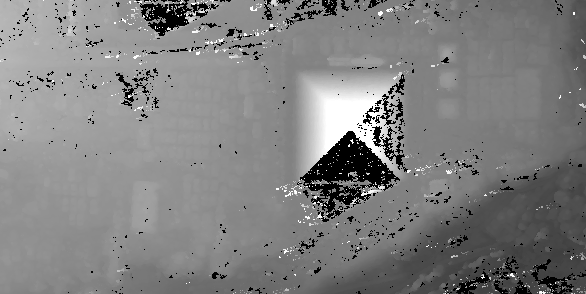
\includegraphics[width=0.7\textwidth]{../Art/MonteverdiImages/stereo_dem_zoom.png}
  \itkcaption[Example]{Extract of the elevation map over Pyramids of Cheops.}
  \label{fig:MeanShiftVectorImageFilter}
\end{figure}
